
\label{cha:res}
% \section{Verdunstungsexperiment}
% \label{res:eva}
% 
% \subsection{Präsentation}
% \label{res:eva:pres}
% 
% \widegraph[./plot/plot_eva]{Das Verdunstungsexperiment (a) zu Beginn der Messung und (b) am Ende nach 16 Tagen und 1,5 Stunden. Die Aufnahmen enstanden in Kombination mit einem \SI{630}{\nano\meter}-Filter. Die Ausbreitung den \BB Tracers ist mit einer weißen gestrichelten Linie bei (b) und (c) eingezeichnet. (c) Zeigt die Differenz der beiden Bilder (siehe Teil \ref{sec:ima}), normiert auf den Wertebereich $(0,\dots,100)$. Man kann erkennen, dass die Zelle im Verlauf der Messung gekippt ist (rote und blaue Streifen im oberen Teil des Bildes).}{fig:reseva}
% 
% 
% Das Verdunstungsexperiment wurde über einen Zeitraum von 16 Tagen und 1,5 Stunden durchgeführt. In Abbildung \ref{fig:reseva} kann man das Ergebnis der Messung sehen. Klar zu erkennen ist, dass sich der \BB-Tracer weit nach oben ausgebreitet hat, ca. über die Hälfte der Zelle. Bevorzugt wurde dabei der Weg über die Mitte der Zelle, was an der keilartigen struktur der Tracerausbreitung ausgemacht wird. 
% 
% Mit Hilfe der Differenzenmethode aus Teil \ref{sec:ima} und durch betrachten der Abfolge aller aufgenommener Bilder in Form eines Films, lässt sich erkennen, dass die Zelle über den Zeitraum des Experiments leicht nach vorne gekippt ist. Dadurch bilden sich rote und blaue Linien aus, da die flaschen Regieonen voneinander abgezogen werden. Eine Abschätzung, wie der Tracer sich ausgebreitet hat ist dennoch in Kombination mit der Originalaufnahme sehr gut möglich und reicht für die qualitative Abschätzung, wie sie hier erfolgen soll.
% 
% 
% \subsection{Schlussfolgerungen}
% \label{res:eva:disk}
% 
% Eine sehr grobe Abschätzung der Menge, des verdunsteten Wassers kann über die Fläche, die der Tracer einnimmt gemacht werden. So wie sie hier durchgeführt wird, kann und soll sie keine harten wissenschaftlichen Daten liefern, aber in Zahlen fassen, was man intuitiv sieht.
% 
% Unter der Annahme, dass die Kügelchen in der Zelle so dicht wie möglich gepackt sind ist die Porosität an allen Stellen $\bar{\phi} = 0,35$. Diese Annahme stellt natürlich eine untere Grenze dar, da die Kugeln nicht perfekt liegen. 
% Die eingenommene Fläche wird mit $\frac{1}{3}$ der Zellenfläche abgeschätzt. Zusammen mit den Abmessungen der Zelle (Tabelle \ref{tab:hsc}) erhält man das abgeschätzte Volumen $V_w$ des verdunsteten Wassers:
% \begin{align}
%  V_{HS-Zelle} &=  \SI{0,4095}{\liter} \\
%  \Rightarrow V_{w} &= \frac{\bar{\phi}}{3} \cdot V_{HS-Zelle} = \SI{0,04778}{\liter}
% \end{align}
% Teilt man dieses Ergebnis durch die Zeitdauer des Experiments erhält man eine Abschätzung für die Verdunstungsrate:
% \begin{align}
%  \dot{V_w} = \SI{0.1239}{\milli\liter\per\hour}
% \end{align}
% 
% \TODO{Vergleich Arbeit Apple}



% \newpage
\section{\COTm Experiment}
\label{res:cot}

\graph{Foto des Aufbaus. Mit roten Rechtecken sind die Bereiche zur Stabilisierung der Helligkeit (oben rechts) und zur tatsächlichen Auswertung (unten) markiert. Von oben kommt der Schlauch, durch welchen das \COT zugeführt wird ins Bild.}{fig:fotoau}

Wie in Teil \ref{cha:set} beschrieben wurde das \COTm Experiment mit der kleinen \HSC durchgeführt. Ein Foto des Aufbaus ist in Abbildung \ref{fig:fotoau} zu sehen. Dort sind auch der Bereich zur Stabilisierung der Helligkeit und der für die Messungen analysierte Bereich eingezeichnet.

Zunächst werden die gemachten Beobachtungen geschildert, anschließend werden sie interpretiert und diskutiert.


\subsection{Beobachtungen}
\label{res:cot:beob}

\sisetup{
  round-mode=places,
  round-precision=1
}


% ========================= Allgemeiner Verlauf =========================
In den Abbildungen \ref{fig:fft} bis \ref{fig:complete} sind die Ergebnisse des \COTm Experiments festgehalten. Die Gesamtdauer des Experiments beläuft sich auf \mbox{\SI{5}{\hour} \SI{6}{\minute}}, der für diese Arbeit interessante Übergang zur Fingerbildung findet nach \SI{9}{\minute} statt. Nach ca. \SI{1,5}{\hour} wird das Verhalten zunehmend von Vortizitäten auf Zellskala dominiert, weshalb spätestens hier alle in Teil \ref{cha:meth} beschriebenen Methoden versagen. 
Die Vortizitäten auf Zellskala sorgen für Durchmischung, da durch sie die Finger nicht mehr gerade nach unten sinken können, sondern zur Seite driften, wo sie wieder nach oben gedrückt werden.

Wie erwartet kann sehr gut die Fingerbildung beobachtet werden. Abbildungen \ref{fig:vcot_1-1}, \ref{fig:vcot_1-2} und \ref{fig:vcot_1-grey} zeigen ihren zeitlichen Verlauf.


% ========================= fft & k_space =========================
\widegraph[./plot/plots_data-1/fft]{Die mit Hilfe der diskreten Fourieranalyse vom Rauschen bereinigten mittleren Intensitäten der Finger. Der zeitliche Verlauf ist farblich codiert und geht von \SI{0}{\minute} (hellblau) bis \mbox{\SI{1}{\hour} \SI{24}{\minute}} (pink).}{fig:fft}

\graph[./plot/plots_data-1/k_space]{Mit Hilfe der diskreten Fourieranalyse bestimmte Abstände (hier in der Einheit $\si{Finger \per \centi\meter}$) der Finger. Man kann gut erkennen, dass dieser bei $k \approx \SI[round-precision=2]{0,66}{\per\centi\meter}$ liegt. Der zeitliche Verlauf ist farblich codiert und geht von \SI{0}{\minute} (hellblau) bis \mbox{\SI{1}{\hour} \SI{24}{\minute}} (pink).}{fig:k_space}

Zur Fingerdetektion wurde, wie beschrieben, eine Fourieranalyse der mittleren Fingerintensitäten durchgeführt (siehe Teil \ref{sec:dec}). Die resultierenden Spektren der Wellenzahlen $k(t)$ sind in Abbildung \ref{fig:k_space} zu sehen. Hier kann man erkennen, dass über den ersten Zeitbereich des Experiments zwischen \SIrange{9}{50}{\minute}, ein Abstand von \SI[round-precision=2]{1,517}{\centi\meter} ($\Rightarrow k=\SI[round-precision=2]{0,66}{\per\centi\meter}$) zwischen den Fingern dominiert und im zeitlichen Verlauf stabil bleibt. 

Der zeitliche Verlauf der mit Hilfe dieser Fourieranalyse bereinigten mittleren Fingerintensitäten ist in Abbildung \ref{fig:fft} dargestellt. Es wurden alle Signale mit einer Wellenzahl $k > \SI{2}{\per\centi\meter}$ als Rauschen eingestuft und ausgefiltert. Hier kann man gut das Wachstum der Finger, in Form der steigenden Amplitude, erkennen, sowie die Bewegung der Finger. %, die relativ konstant bleibt. 

% ========================= Fingerzahl =========================
% \graph[./plot/plots_data-1/fcount]{Anzahl der detektierten Finger im Verlauf des Experiments. Das Rauschen tritt auf, da die Methode nicht einwandfrei funktioniert. Siehe dazu auch \ref{fig:f_detect}. Im Zeitraum von \SIrange{9}{40}{\minute} liefert sie allerdings relativ verlässliche Ergebnisse.}{fig:fcount}

\graph[./plot/plots_data-1/fgrowth]{Länge der detektierten Finger im Verlauf des Experiments. Das Rauschen tritt auf, da die Methode nicht einwandfrei funktioniert. Siehe dazu auch \ref{fig:f_detect}. Im Zeitraum zwischen \SIrange{9}{40}{\minute} liefert sie allerdings relativ verlässliche Ergebnisse.}{fig:fgrowth}

% Die Graphen \ref{fig:fcount} und \ref{fig:fgrowth} zeigen Zahl und mittlere Länge der Finger über den Verlauf der Messung. 
Der Graph \ref{fig:fgrowth} zeigt die mittlere Länge der Finger im Verlauf der Messung. Für diese Betrachtung wurde der untersuchte Bereich der \HSC in 9 gleich große Teile aufgeteilt und über die Längen der Finger in diesen Bereichen gemittelt, um zu sehen, ob das Wachstum in verschiedenen Bereichen der Zelle unterschiedlich ist.
Hier zeigt sich, was auch in Abbildung \ref{fig:vcot_1-1} zu erkennen ist: die Länge der Finger nimmt relativ linear mit verlauf der Zeit zu.

% einzelner Finger
Für generauere Betrachtung des Übergangs vom diffusiven zum konvektiven Vermischungsprozess von Wasser und \COT sind in Abbildung \ref{fig:vcot_1-grey} und \ref{fig:sevo} die ersten \SI{16}{\minute}, bzw. \SI{52}{\minute} des Experiments gezeigt. Hierfür wurden die originalen Aufnahmen verwendet, da man hier deutlicher den Effekt beobachten kann.

Man kann erkennen, dass im Verlauf des Experiments, zwischen \SI{5}{\minute} und \SI{9}{\minute} der Übergang stattfindet. Anschließend bilden sich zunächst schnell, ab \SI{24}{\minute} etwas langsamer Finger aus. Direkt zu Beginn der Fingerbildung kann man sehen, wie die diffusive Schicht abgesaugt wird, ebenso wie kürzere Finger. Dies wird in Abbildung \ref{fig:sevo} (\SIrange{9}{26}{\minute}) besonders deutlich. In diesem Zeitraum kann man beobachten, wie rechts und links von dem am größten hervorragenden Finger die diffusive Schicht kleiner wird, bis sie fast wieder reines Wasser an der Wasseroberfläche ist. Nach \SI{24}{\minute} ist die obere \COT Schicht wieder so dick wie nach \SI{9}{\minute}. Nach \SI{39}{\minute} sorgen Vortizitäten dafür, dass die Schicht wieder dünner und vom Finger abgeleitet wird.

Letztendlich verschmelzen immer mehr Finger miteinander und es gibt nach einer Stunde immer weniger Finger (siehe \zB Abbildung \ref{fig:complete}). Diese wandern entlang der Wasseroberfläche.
Nach \SI{5}{\hour} ist die Zelle sehr gut, wenn auch noch nicht komplett, durchmischt.


\subsection{Diskussion}
\label{res:cot:disk}

Ein Vergleich der oben gezeigten Ergebnisse mit denen aus anderen Arbeiten zeigen gute Übereinstimmungen.
\cite{kneafsy} beschreiben in Ihrer Arbeit die \COTm Sequestration, so wie sie auch hier zu beobachten ist. Auch dort wird der Effekt beobachtet, dass die diffusive Schicht, welche sich zunächst ausbildet, mit Entstehen der Finger dünner wird.

Grund für dieses Verhalten ist die Konvektion des \COTm haltigen Wassers (siehe Abbildung \ref{fig:difkon}). 
% Durch die Abwärtsbewegung dieser dichteren Lösung, wird klares Wasser von unten nach oben transportiert. Dieses kann nun wieder leichter \COT aufnehmen, im Vergleich zum Wasser, in dem sich bereits \COT gelöst hat und damit ggf. schon gesättigt ist.

Was beobachtet werden kann sind zwei Prozesse, die einander beeinflussen: 
\begin{itemize}
 \item Mittels Diffusion wird das gelöste \COT langsam in tiefere Wasserschichten gebracht.
 \item Sobald die dadurch ausgebildete Schicht instabil wird, brechen Finger hervor. Es beginnt ein konvektiver Prozess, der das gelöste \COT schneller in noch tieferes Wasser bringt.
 \item Dadurch wiederum gelangt reines Wasser an die Oberfläche, was wiederum die Lösung von \COT im Wasser begünstigt.
 \item Neues \COT wird im Wasser gelöst und über die Konvektionskanäle, also die Finger, abtransportiert.
\end{itemize}

Das Verhalten der Finger, das nach spätestens \SI{50}{\minute} zu beobachten ist, lässt sich allerdings damit nicht erklären. Da die Zelle endlich tief ist, entstehen durch die Abwärtsbewegung des gelösten \COT Kreisströme in Größenordnung der Zellentiefe. Diese führt dazu, dass die Finger nach außen driften und gelöstes \COT wieder nach oben transportiert wird.
 
Die stabilen Abstände zwischen den Fingern, in den ersten \SI{50}{\minute}, lassen sich auch durch die konvektiven Prozesse zu Beginn erklären. Diese wirken stabilisierend auf die Finger, solange keine Vortizitäten auf Zellskala auftreten.
Intuitiv macht es Sinn, dass die Abstände der Finger in Größenordnung ihrer Breite sein sollte, da das durch die Finger verdrängte Volumen dem nach oben gedrängten entsprechen muss. Dieses Verhalten wird beobachtet.
Ähnliche Beobachtungen zur Stabilisierung der Fingersabstände werden von \cite{fernandez} gemacht. Auch dort dominiert ein Abstand zu Beginn der Fingerbildung. 

Damit lässt sich das Experiment insgesamt in drei Phasen gliedern:
\begin{itemize}
 \item Diffusion (\SI{0}{\minute} bis \SI{9}{\minute})
 \item stabile Fingerbildung (\SI{9}{\minute} bis \SI{60}{\minute})
 \item Vortizitäten auf Zellebene (\SI{60}{\minute} bis zum Ende) 
\end{itemize}


Bei der Auswertung dieser Messung gibt es mehrere bekannte Fehlerquellen, die an dieser Stelle Erwähnung finden sollen. Zum einen sind die Aufnahmen, aufgrund der niedrigen Belichtungszeit verrauscht, was die Fingerdetektion und -längenmessung, trotz Vorkehrungen, fehleranfällig macht.

Weitaus größeres Problem ist allerdings das Schwanken der Belichtung der Kamera. Leider konnte nicht hersausgefunden werden, woher dieser Effekt kommt. Was man feststellen kann ist, dass die Kamera im Laufe der Zeit immer dunklere Bilder macht. Dieser Effekt sollte, durch die in Teil \ref{sec:ima} beschriebene Methode zur Korrektur der Helligkeitsschwankungen, ausgeglichen werden. Leider konnte die angewandte Methode allerdings, aus unverstandenen Gründen, nicht die gewünschten Ergebnisse liefern. Die Helligkeit der Bilder schwankt trotz allem, wenn auch weniger stark. Dennoch führt dies dazu, dass, wie man in Abbildung \ref{fig:vcot_1-1} sehen kann, die Intensitäten der Finger schwanken und schwächer werden. Auch das führt zu fehlerhaften Längenbestimmungen der Finger, da der Grenzwert (siehe Teil \ref{sec:lan}) zu spät erreicht wird.

Diese Fehlerquellen wirken sich aber nicht negativ auf die Bestimmung der Fingerabstände über die Fourieranalyse aus. Da die mittlere Intensitäten, trotzdem das charakteristische Wellenmuster (siehe Abbildung \ref{fig:fft}) aufweisen. Die Aussagen aus, welche diesen Messungen gewonnen wurden sind somit robuster.

\graph[./plot/Konvektion_Diffusion.pdf]{Interpretation der auftretenden Phänomene, verursacht durch Konvektion und Diffusion}{fig:difkon}


% \onecolumn
% 
% \begin{figure}
%  \centering
%  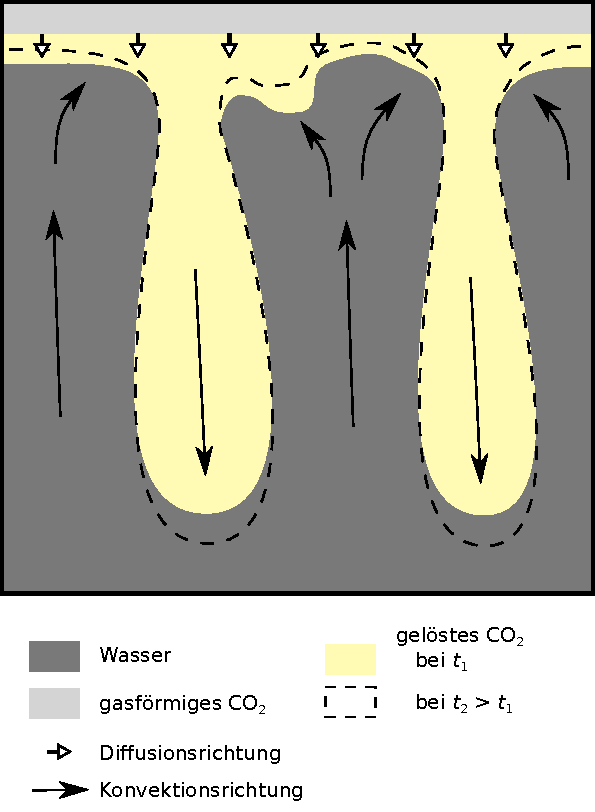
\includegraphics[width=9cm]{./plot/Konvektion_Diffusion.pdf}
%  \caption{Interpretation der auftretenden Phänomene, verursacht durch Konvektion und Diffusion}
%  \label{fig:difkon}
% \end{figure}
% 
% \twocolumn


% \newpage
% \mbox{\,}
\newpage

\section{\COTm Experiment mit porösem Medium}
\label{res:cpm}

\graph[./plot/BCG_test_03_num]{Farbumschläge des \BCG in Verbindung mit verschiedenen Substanzen. \BCG (1) in neutraler Form, \dah im Gleichgewicht mit der umgebenden Luft, (2) in Kombination mit \COT. Man kann sehr gut den Ausschlag ins Gelbe erkennen. (3) mit den Glaskügelchen verschiedener Größen, (4) mit Glaskügelchen und gelöstem \COT.}{fig:CPO}

\graph[./plot/BCG_Test_Boro_num]{Farbumschläge des \BCG. \BCG (1) in neutraler Form, \dah im Gleichgewicht mit der umgebenden Luft, (2) in Kombination mit gelöstem \COT. Man kann sehr gut den Ausschlag ins Gelbe erkennen. (3) mit den Glaskügelchen aus Borosilikatglas, (4) mit Glaskügelchen und gelöstem \COT.}{fig:CPO_bor}

Der Versuch das \COT Experiment in Kombination mit einem porösen Medium durchzuführen ist aufgrund der verwendeten Glaskugeln gescheitert. Es wurde nicht beachtet, dass Glas Wasser durch Ionenaustausch basisch macht. Die leicht löslichen Elemente an der Oberfläche des Glases werden vom Wasser herausgelöst und durch die im Wasser vorhandenen H$^+$-Ionen ersetzt. Dadurch wird das Wasser basisch, da die OH$^-$-Konzentration steigt. \citep{Vogel}

Dieser Effekt ist durch die große Oberfläche, die die Kügelchen insgesamt haben, nicht zu vernachlässigen und sorgt dafür, dass der benutze Indikator nur den basischen Farbton annimmt. Das Lösen von \COT im Wasser kann diesen Effekt offensichtlich nicht überwiegen.

Zur Verdeutlichung der beschriebenen Phänomene siehe Abbildung \ref{fig:CPO}.

Ein angedachter Lösungsansatz mit Glaskugeln, welche dem Wasser gegenüber beständiger sind, wurde aus Zeitgründen nicht umgesetzt. Ein Test der Kugeln aus Borosilikatglas ergab aber vielversprechende Ergebnisse, da der durch das \COT hervorgerufene Farbumschlag auch mit Kugeln in der Indikatorlösung beobachtet werden konnte. Siehe dazu Abbildung \ref{fig:CPO_bor}.

% \vspace{10cm} % damit balance die Bilder beide auf die Seite packt



  
% ========================= longgraphpages =========================
\longgraphpage[./plot/plots_data-1/plot_all_overview_quot_0]{Fingerbildung Experiment 1. Die Farbskala beschreibt die relative Absorption im Bezug auf den Hintergrund (0). Maximale Absorption bekommt den Wert 100 zugewiesen.}{fig:vcot_1-1}
\longgraphpage[./plot/plots_data-1/plot_all_overview_quot_1]{Fingerbildung Experiment 1. Die Farbskala beschreibt die relative Absorption im Bezug auf den Hintergrund (0). Maximale Absorption bekommt den Wert 100 zugewiesen.}{fig:vcot_1-2}

\longgraphpage[./plot/plots_data-1/finger_detection_cut]{Abgebildet sind Fingerbildung zusammen mit detektierten Fingerpositionen und -längen zur Demonstration, wie die in Teil \ref{sec:lan} beschriebene Methode funktioniert. Die Farbskala beschreibt die relative Absorption im Bezug auf den Hintergrund (0). Maximale Absorption bekommt den Wert 100 zugewiesen.}{fig:f_detect}


\longgraphpage[./plot/plots_data-1/plot_all_overview_0_adj]{Fingerbildung Experiment 1. Rohaufnahmen mit erhöhtem Kontrast. Zu erkennen ist der Übergang vom diffusiven zum konvektiven Prozess nach ca. \SI{9}{\minute}. Auch kann man beobachten, wie die diffusive Schicht zwischen den Fingern ``abgesaugt'' wird. }{fig:vcot_1-grey}
% ========================= einzelner Finger =========================
\longgraphpagetriple{./plot/plots_data-1/single_evolution_1}{./plot/plots_data-1/single_evolution_2}{./plot/plots_data-1/single_evolution_3}{Entwicklung eines einzelnen Fingers mit der Zeit.}{fig:sevo}

\longgraphpagesextuple{./plot/plots_data-1/comp_evolution_1}{./plot/plots_data-1/comp_evolution_2}{./plot/plots_data-1/comp_evolution_3}{./plot/plots_data-1/comp_evolution_4}{./plot/plots_data-1/comp_evolution_5}{./plot/plots_data-1/comp_evolution_6}{Überblick über den gesamten Verlauf des Experiments}{fig:complete}
% \widegraphpage[./plot/plots_data-1/fingers_quot-raw_5-30_cut.png]{Vergleich der Quotientenmethode und dem tatsächlich aufgezeichneten Bild.}{fig:fing_comp}
